\documentclass[10pt,a4paper]{ctexart}
\usepackage[margin=2cm]{geometry}
\usepackage{graphicx}
\usepackage{hyperref}
\usepackage{amsmath}    % 提供方程环境
\usepackage{physics}    % 简化向量、微分算子语法
\newcommand{\myspace}[1]{\par\vspace{#1\baselineskip}} %自定义空一行
\usepackage{fancyhdr}
\usepackage{wrapfig}
\usepackage{booktabs} % 添加 booktabs 宏包
\pagestyle{fancy}
\fancyhf{}  % 清除所有页眉页脚
\fancyfoot[C]{\thepage}  % 在页脚中央设置页码
\renewcommand{\headrulewidth}{0pt}  % 去掉页眉横线
\renewcommand{\footrulewidth}{0pt}  % 去掉页脚横线

\usepackage{hyperref}
\hypersetup{
    colorlinks=true,
    linkcolor=blue,
    filecolor=magenta,      
    urlcolor=cyan,
    pdftitle={Overleaf Example},
    pdfpagemode=FullScreen,
    }

\usepackage{titlesec}

% 重新定义section格式
\titleformat{\section}
  {\normalfont\Large\bfseries}
  {\chinese{section}、}
  {0pt}
  {}

% 给出常用字号的自定义指令
\newcommand{\chuhao}{\fontsize{42pt}{48pt}\selectfont}
\newcommand{\xiaochu}{\fontsize{36pt}{42pt}\selectfont}
\newcommand{\xiaoer}{\fontsize{18pt}{21.6pt}\selectfont}
\newcommand{\sanhao}{\fontsize{16pt}{20pt}\selectfont}
\newcommand{\xiaosan}{\fontsize{15pt}{18pt}\selectfont}
\newcommand{\sihao}{\fontsize{14pt}{18pt}\selectfont}
\newcommand{\xiaosi}{\fontsize{12pt}{16pt}\selectfont}
\newcommand{\wuhao}{\fontsize{10.5pt}{12.6pt}\selectfont}

% 定义中文数字转换
\titleformat{\section}
  {\normalfont\Large\bfseries}
  {\zhnum{section}、}  % 使用\zhnum而不是\chinese
  {0pt}
  {}

% 标题设置
\title{\xiaochu\textbf{物理实验预习报告}}
\author{}
\date{}

\begin{document}

\vspace*{36pt} % 顶部空白

% 居中填写区域
\begin{center}
    
\includegraphics[width = 9cm]{figures/head.png}
    
    \xiaochu\textbf{物理实验预习报告}
    % 预留空白区域
    \vspace{13pt}
    \vspace{13pt}
    \vspace{13pt}
    \vspace{13pt}
    
    \sanhao\textbf{实验名称：\underline{\makebox[8cm]{ 双棱镜干涉实验 }}} \\[10pt]
    \sanhao\textbf{实验桌号：\underline{\makebox[8cm]{  }}} \\[10pt]
    \sanhao\textbf{指导教师：\underline{\makebox[8cm]{ }}} \\[20pt]
    
    % 预留空白区域
    \myspace{7}
    
   \sihao\textbf{班级：\underline{\makebox[6cm]{cc98}}} \\[10pt]
    \sihao\textbf{姓名：\underline{\makebox[6cm]{Hydrofoil}}} \\[10pt]
    \sihao\textbf{学号：\underline{\makebox[6cm]{324010}}} \\[30pt]
    
    \sihao\textbf{实验日期: \underline{\makebox[0.8cm]{2026}}年 \underline{\makebox[0.4cm]{1}}月\underline{\makebox[0.4cm]{5}}日  星期\underline{\makebox[0.6cm]{一}}上午}
    
    \vspace{18pt}
    \sihao 浙江大学物理实验教学中心
    
\end{center}

\newpage


    \section{实验综述}
    
    \xiaosi （自述实验现象、实验原理和实验方法，不超过500字，5分）
    
\begin{wrapfigure}{r}{0.4\textwidth}
    \centering
         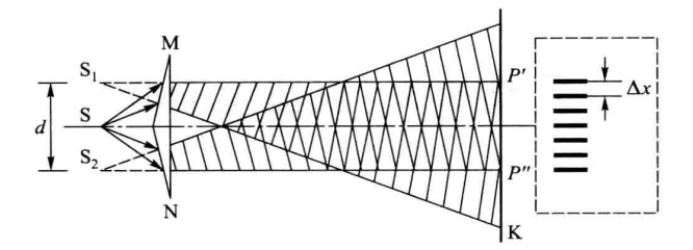
\includegraphics[width=8cm]{figures/1.png} 
    \caption{双棱镜干涉原理示意图}
    \label{fig:principle}
    \end{wrapfigure}

    \

    \subsubsection*{双棱镜干涉原理:}

    菲涅耳双棱镜实验属于分波前干涉。双棱镜由两块底面重合的直角棱镜构成，具有极小的楔角（通常 $<1^\circ$）。当单色线光源（狭缝 $S$）发出的光波入射到双棱镜上时，经过棱镜的两次折射，光束被分成两部分，分别通过棱镜的上半部和下半部。这两束光看起来像是从两个虚光源 $S_1$ 和 $S_2$ 发出的。由于 $S_1$ 和 $S_2$ 均来自同一个实际光源 $S$，它们满足相干条件（频率相同、振动方向相同、相位差恒定）。
    
    在双棱镜后方的重叠区域（干涉场）内，来自 $S_1$ 和 $S_2$ 的相干光发生干涉，形成明暗相间、等间距的平行直条纹。
    
    \subsubsection*{光波波长测定原理:}

     \begin{wrapfigure}{r}{0.4\textwidth}
    \centering
         
\includegraphics[width=8cm]{figures/图片2.png} 
    \caption{波长测定原理示意图}
    \label{fig:principle}
    \end{wrapfigure}


    在双棱镜干涉实验中，通过测量干涉条纹间距来计算光波波长。
    如图所示，设两个虚光源 $S_1$ 和 $S_2$ 之间的距离为 $d$，它们到光屏（测微目镜焦平面）的距离为 $D$。考察屏上某一点 $P$，其偏离中心的距离为 $x$。
    
    根据杨氏干涉原理，两束相干光到达点 $P$ 的光程差 $\delta$ 可近似表示为：
    \begin{align*}
        \delta \approx d \sin \theta \approx d \frac{x}{D}
    \end{align*}
    
    对于第 $k$ 级暗纹，其位置记为 $x_k$，光程差 $\delta_k$ 满足：
    \begin{align*}
        \delta_k = d \frac{x_k}{D}
    \end{align*}
    
    对于相邻的第 $k+1$ 级暗纹，其位置记为 $x_{k+1}$，光程差 $\delta_{k+1}$ 满足：
    \begin{align*}
        \delta_{k+1} = d \frac{x_{k+1}}{D}
    \end{align*}
    
    相邻两级暗纹的光程差之差应为一个波长 $\lambda$（即 $\delta_{k+1} - \delta_k = \lambda$），代入上式可得：
    \begin{align*}
        \lambda = \frac{d}{D} (x_{k+1} - x_k)
    \end{align*}
    
    令相邻条纹间距 $\Delta x = x_{k+1} - x_k$，整理即得波长测定公式：
    \begin{align*}
        \lambda = \frac{d}{D} \Delta x
    \end{align*}
    
    实验中，通过测微目镜测出 $\Delta x$，并配合二次成像法测出 $d$ 和 $D$，即可计算出待测光波的波长 $\lambda$。

    \subsubsection*{二次成像法测量虚光源间距 $d$:}

    \begin{wrapfigure}{r}{0.4\textwidth}
    \centering
         
\includegraphics[width=6cm]{figures/图片1.png} 
    \caption{二次成像法原理示意图}
    \label{fig:principle}
    \end{wrapfigure}

    由于虚光源 $S_1$ 和 $S_2$ 是不可见的，直接测量其间距 $d$ 较为困难且误差较大。本实验采用“二次成像法”（Bessel法）借助凸透镜进行间接测量。
    
    在狭缝与光屏距离 $D$ 保持不变（且 $D > 4f$，其中 $f$ 为凸透镜焦距）的情况下，移动凸透镜，可以在光屏上找到两个位置，使虚光源 $S_1, S_2$ 分别成清晰的实像。
    
    1. 当透镜靠近狭缝时，成放大的实像，测得两像间距为 $d_1$；
    2. 当透镜靠近光屏时，成缩小的实像，测得两像间距为 $d_2$。
    
    根据几何光学放大率关系，可推导出虚光源间距 $d$ 为：
    \begin{align*}
        d = \sqrt{d_1 d_2}
    \end{align*}
    
    同时，通过透镜成像公式，可利用光具座上的读数精确测量距离参数。本实验中，通过测量干涉条纹间距 $\Delta x$ 以及 $d_1, d_2$ 和 $D$，即可计算出激光波长 $\lambda$。
   
    
    \section{实验重点}

    \xiaosi（简述本实验的学习重点，不超过100字，3分）


     \begin{enumerate}   
        \item 掌握分波前干涉（双棱镜干涉）的基本原理；
        \item 掌握光路共轴调节技巧，特别是激光束、狭缝、双棱镜主截面的对准；
        \item 理解并运用二次成像法（Bessel法）间接测量虚光源间距 $d$；
        \item 熟练使用测微目镜精确测量细小的干涉条纹间距。
    \end{enumerate}  
    
    
    \section{实验难点}
    
    \xiaosi（简述本实验的实现难点，不超过100字，2分）

    \begin{enumerate}    
        \item \textbf{光路调节难}：需确保狭缝方向与双棱镜棱脊严格平行，否则干涉条纹模糊或倾斜；同时需调节系统共轴，保证光斑打在各元件中心。
        \item \textbf{干涉图样寻找}：双棱镜折射角很小，干涉区域窄，需细致调节前后距离和横向位置才能在目镜中观察到清晰条纹。
        \item \textbf{微弱信号观测}：二次成像中，缩小像的光强较弱且间距小，容易被背景杂散光干扰，需仔细辨别。
        \item \textbf{空程差消除}：使用测微目镜测量条纹间距时，必须单向旋转鼓轮以消除螺距空程差。
    \end{enumerate}  \



\newpage

\sihao\textbf{注意事项：}
\xiaosi
\begin{enumerate}
    \item  用 PDF 格式上传“实验报告”，文件名：学生姓名+学号+实验名称+周次。
    \item  “实验报告”必须递交在“学在浙大”的本课程的对应实验项目的“作业”模块内。
    \item  “实验报告”成绩必须在“浙江大学物理实验教学中心网站”-“选课系统”内查询。
    \item 教学评价必须在“浙江大学物理实验教学中心网站”-“选课系统”内进行，学生必须进行教学评价，才能看到实验报告成绩，教学评价必须在本次实验结束后 3 天内进行。
\end{enumerate}

\vspace{1cm}
\xiaosi\centering \textbf{浙江大学物理实验教学中心制}

\end{document}